\documentclass{article}
\usepackage[utf8]{inputenc}
\usepackage{pgfplots}

\begin{document}
\begin{figure}

\begin{center}

    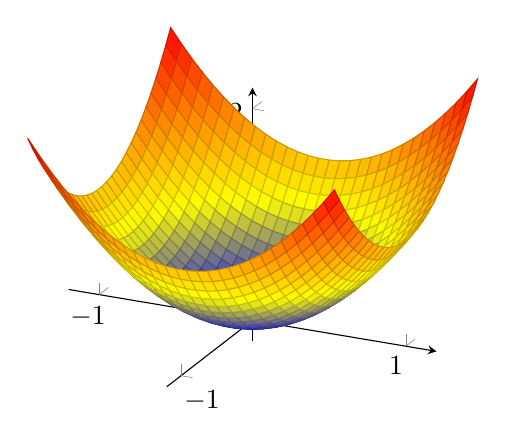
\begin{tikzpicture}[
    declare function = {
        %q(\x) = 5*\x - 1;
        Z(\x,\y) = x^2+y^2; %+ q(\x);
    }]
    \begin{axis}
       [
       axis lines=center,
       enlargelimits,
       tick align=inside,
       domain=-1:1,
       samples=30, 
       %minor tick num=7,
       ]
       \addplot3 [surf] {Z(x,y)};
       %\draw [thick, -latex] (0,0) to [bend right] (0,3);
      % \draw[dashed,line width=0.005\linewidth, ->] (axis cs:-1.1, 1.35, 1) -- (axis cs:0.0,-0.2,0.65);
    \end{axis}
    \end{tikzpicture}
\end{center}
    \caption{Convex Function $f(x,y) = x^2 + y^2$.}
\end{figure} 


\end{document}